\section{Feedforward Neural Networks}
\label{sec:feedforward_neural_networks}
A natural extension of the perceptron model is to combine multiple perceptrons in a network architecture. It is intuitively clear that, much like in an organic brain, a complex arrangement of many simple computing units can learn much more complicated functions than those simple units alone. In this section, we will examine how such a network architecture based on perceptrons can be constructed. The ideas that we develop are mostly based on Ref. \cite[Ch.\,6]{DBLP:books/daglib/0040158}.

\subsection{Extensions to the Perceptron}
Before explaining the composition of perceptrons to neural networks, we will first explore two extensions to the perceptron model that are common in neural networks.

First, we introduce an additional term called \emph{bias} to the output calculation. The new output $\hat{y}$ becomes
\begin{equation}
\hat{y} = \sign(\bm{w}^\top\bm{x} + b),
\end{equation}
where the scalar $b$ is the bias. This additional learnable parameter shifts the function computed by the model independently of its input. If the bias is large and positive, the model is more inclined to predict a positive label, while a negative bias makes it more likely that negative labels are predicted.

Second, we generalize the perceptron by replacing the $\sign$ function with an arbitrary function $f$ called \emph{activation function}. In contrast to $\sign(x)$, most activation functions used in neural networks are continuous, since this enables us to use a variety of \emph{gradient-based} learning algorithms for training as we will see in Section \ref{sec:training}. Concrete examples of activation functions will be discussed later in this section.

Since we will sometimes need the weighted input without the activation function, we also introduce the intermediate quantity

\begin{equation}
z = \bm{w}^\top\bm{x} + b.
\end{equation}

The computing units we have obtained with these modifications to the perceptron are generally called \emph{neurons} or simply \emph{units}.

\begin{comment}
One common activation function is the \emph{logistic sigmoid}:

\begin{equation}
\sigma(x) = \frac1{1+e^{-x}}.
\end{equation}

\begin{figure}
	\begin{center}
		% !TeX root = dm-template.tex

% restrict y to domain=-1:1, x=1cm
\begin{tikzpicture}[scale=.9]
	\begin{axis}[axis lines = left,xlabel = $x$, ylabel = {$\sigma(x)$}, ymin=-0.05, ymax=1.05]
		\addplot [domain=-6:6, samples=200, color=blue, style=semithick]
		{1/(1+exp(-x))};
		%\addlegendentry{$\sigma(x) = 1/\exp(-x)$}
	\end{axis}
\end{tikzpicture}
	\end{center}
	\caption{The logistic sigmoid function.}
	\label{fig:sigmoid}
\end{figure}

As shown in Fig. \ref{fig:sigmoid}, $\sigma(x)$ squashes the output to a value between 0 and 1. A very similar function, producing an output between -1 and 1, is $\tanh(x)$. Lastly, one of the most commonly used activation functions is the \emph{rectified linear} function $g(x) = \max\{0,x\}$ plotted in Fig. \ref{fig:relu}.

\begin{figure}
	\begin{center}
		% !TeX root = dm-template.tex

% restrict y to domain=-1:1, x=1cm
\begin{tikzpicture}[scale=.9]
	\begin{axis}[axis lines = left,xlabel = $x$, ylabel = {$g(x)$}, ymin=-0.5]
		\addplot [domain=-8:8, samples=200, color=blue, style=semithick]
		{max(0,x)};
		%\addlegendentry{$\sigma(x) = 1/\exp(-x)$}
	\end{axis}
\end{tikzpicture}
	\end{center}
	\caption{The rectified linear function.}
	\label{fig:relu}
\end{figure}

The choice of activation function is an important design decision that can greatly influence how well the model learns. The rectified linear function is a very good default choice, as it has shown to outperform other functions in a variety of different model architectures \cite{DBLP:journals/jmlr/GlorotBB11 ,DBLP:conf/nips/KrizhevskySH12}. We will see why some functions work better than others in Section \ref{sec:training}.
\end{comment}

\subsection{Network architecture}
Any arrangement of neurons in a network architecture can be considered a neural network. The most influential such architecture is the feedforward neural network, which forms the basis for many other more advanced neural networks \cite[Ch.\,6,\,p.\,163]{DBLP:books/daglib/0040158}. Feedforward neural networks are sometimes also called \emph{multilayer perceptrons} (MLPs).

In feedforward neural networks, the computing units are arranged in layers. We distinguish between the \emph{output layer}, the \emph{hidden layers}, and the \emph{input layer}. The output layer is the final layer in the network were its actual output is produced. The input layer is the first layer in the network, and all layers in between are called hidden layers. The input layer is special as it does not compute anything; it merely represents the input that is passed into the neural network. In general, a $L$-layer feedforward neural network consists of one input layer, $L-2$ hidden layers, and an output layer. We call the number of layers $L$ the \emph{depth} of the model.

Every neuron in a layer $l$ receives input from all neurons in the \nth{(l-1)} layer. There are no connections between neurons in the same layer, and we also do not allow feedback connections into previous layers. Neurons in the hidden and output layers behave exactly as the modified perceptron; the only important detail is that their input is the output from the previous layer.

An illustration of a feedforward neural network can be found in Fig. \ref{fig:network}.
\begin{figure}
	\begin{center}
		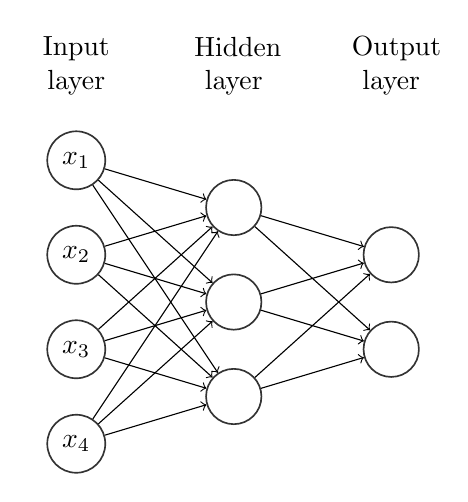
\begin{tikzpicture}
	\tikzstyle{neuron} = [circle,draw=black!80,semithick,minimum size=20pt]
	\tikzstyle{layer} = [text width=1cm, align=center]
	% input layer
	\node[layer] at (0, 0) {Input layer};
	\foreach \i in {1,...,4}
		\node[neuron] (input\i) at (0, -\i*1.2) {$x_\i$};
	% hidden layer
	\node[layer] at (2, 0) {Hidden layer};
	\foreach \i in {1,...,3}
		\node[neuron] (hidden\i) at (2, -\i*1.2 -.6) {};
	% output layer
	\node[layer] at (4, 0) {Output layer};
	\foreach \i in {1,...,2}
		\node[neuron] (output\i) at (4, -\i*1.2 -1.2) {};
	% connections input->hidden
	\foreach \i in {1,...,4}
		\foreach \j in {1,...,3}
			\draw[->] (input\i) -- (hidden\j);
	% connections hidden->output
	\foreach \i in {1,...,3}
		\foreach \j in {1,...,2}
			\draw[->] (hidden\i) -- (output\j);
\end{tikzpicture}
	\end{center}
	\caption{A three-layer neural network. The network accepts an input $\bm{x} \in \mathbb{R}^4$, propagates it through its hidden layer consisting of three units, and finally produces an output $\hat{\bm{y}} \in \mathbb{R}^2$ in the output layer. The weights, sums, and activation functions have been omitted.}
	\label{fig:network}
\end{figure}

In the remainder of this section, we will discuss the individual layers and corresponding design decisions in more detail.

\subsubsection{Output layer}
The design of the output layer depends mostly on the task that we wish to perform with the neural network. If we want to predict a continuous output, a problem known as \emph{regression}, we use a linear output layer where the activation function simply is the identity function. The number of neurons in the output layer is equal to the dimensionality of the output space.

In \emph{classification}, we wish to predict which class an input vector $\bm{x}$ belongs to. For example, as with the perceptron, we might want to distinguish normal emails from spam emails. In this case of \emph{binary} classification, it is common to use the activation function
\begin{equation}
\sigma(x) = \frac1{1+\exp(-x)},
\end{equation}
called the logistic sigmoid, in combination with a single output unit.
\begin{figure}
	\begin{center}
		% !TeX root = dm-template.tex

% restrict y to domain=-1:1, x=1cm
\begin{tikzpicture}[scale=.9]
	\begin{axis}[axis lines = left,xlabel = $x$, ylabel = {$\sigma(x)$}, ymin=-0.05, ymax=1.05]
		\addplot [domain=-6:6, samples=200, color=blue, style=semithick]
		{1/(1+exp(-x))};
		%\addlegendentry{$\sigma(x) = 1/\exp(-x)$}
	\end{axis}
\end{tikzpicture}
	\end{center}
	\caption{The logistic sigmoid function.}
	\label{fig:sigmoid}
\end{figure}
As shown in Fig. \ref{fig:sigmoid}, $\sigma(x)$ squashes its input to a value between 0 and 1, which can be interpreted as a Bernoulli distribution. Thus, it is an excellent choice for binary classification problems: the output of the neural network is the probability that it assigns to one specified class.

In \emph{multiclass} classification problems, where we wish to predict a probability distribution over $k$ different classes, we construct an output layer with $k$ units. A generalization of the logistic sigmoid, called the $\softmax$ function
\begin{equation}\label{eq:softmax}
\softmax(x) = \frac{\exp(x)}{\sum_{i=1}^{k}\exp(z_i)},
\end{equation}
is commonly used as activation function in this scenario. In Eq. \eqref{eq:softmax}, $z_i$ represents the weighted input $z$ of the \nth{i} neuron in the output layer. We can easily see that the $\softmax$ function creates a valid probability distribution and that neurons that have a large weighted input are assigned a higher probability. The output $\hat{y}_i$ of the neural network is the probability it assigns to the \nth{i} class.

\todo[inline]{Other, different tasks: structured output, anomaly, ... cite...}
\subsubsection{Hidden layers}
In contrast to the output layer, the task that we want so solve does not give us any information about how to design the hidden layers. \todo[inline]{Depth, width, harder to train (more parameters), activation functions, linear nonlinear, representation, ...}